%
%                       This is a basic LaTeX Template
%                       for the Informatics Research Review

\documentclass[a4paper,11pt]{article}
% Add local fullpage and head macros
\usepackage{head,fullpage}     
% Add graphicx package with pdf flag (must use pdflatex)
\usepackage[pdftex]{graphicx}  
% Better support for URLs
\usepackage{url}
% Date formating
\usepackage{datetime}

\newdateformat{monthyeardate}{%
  \monthname[\THEMONTH] \THEYEAR}

\parindent=0pt          %  Switch off indent of paragraphs 
\parskip=5pt            %  Put 5pt between each paragraph  
\Urlmuskip=0mu plus 1mu %  Better line breaks for URLs


%                       This section generates a title page
%                       Edit only the following three lines
%                       providing your exam number, 
%                       the general field of study you are considering
%                       for your review, and name of IRR tutor

\newcommand{\examnumber}{B240710}
\newcommand{\field}{Network Science Analysis : An Elixir to Prevent Global Financial Crisis?}
\newcommand{\supervisor}{Xinran Ruan}

\begin{document}
\begin{minipage}[b]{110mm}
        {\Huge\bf School of Informatics
        \vspace*{17mm}}
\end{minipage}
\hfill
\begin{minipage}[t]{40mm}               
        \makebox[40mm]{
        \includegraphics[width=40mm]{crest.png}}
\end{minipage}
\par\noindent
    % Centre Title, and name
\vspace*{2cm}
\begin{center}
        \Large\bf Informatics Research Review \\
        \Large\bf \field
\end{center}
\vspace*{1.5cm}
\begin{center}
        \bf \examnumber\\
        \monthyeardate\today
\end{center}
\vspace*{5mm}

%
%                       Insert your abstract HERE
%                       
\begin{abstract}
The emerging global financial system marked a new era where institutions, markets, and players are interconnected and depending on each other. Although it boosts global economic progress, it is exposed to systemic risk due to its properties. Network science is then proposed to manage such risk because its properties resemble real-world global financial systems. In this review, we explore the multiple usages of network science in global stock markets and draw context of usage, advantages, and disadvantages for each of the methods for future use cases.
\end{abstract}

\vspace*{1cm}

\vspace*{3cm}
Date: \today

\vfill
{\bf Supervisor:} \supervisor
\newpage

%                                               Through page and setup 
%                                               fancy headings
\setcounter{page}{1}                            % Set page number to 1
\footruleheight{1pt}
\headruleheight{1pt}
\lfoot{\small School of Informatics}
\lhead{Informatics Research Review}
\rhead{- \thepage}
\cfoot{}
\rfoot{Date: \date{\today}}
%

\section{Introduction}
In the modern world, the global financial system is an intricate web of institutions, markets, and mechanisms that facilitates the flow of capital, currencies, and financial instruments on a worldwide scale (Investopedia, 2019). As the backbone of the modern global economy, this system connects individuals, businesses, governments, and financial entities across the world, forming a complex network of interactions among them. This network is instrumental for the aforementioned parties in allocating resources, managing risks, and also supporting economic growth on international scale. Over the years, the network evolves following historical developments, technological advancements, and the dynamic nature of financial markets across the globe. Because of the interconnectedness properties of the network, it became the key driver for economic progress and a facilitator for borderless collaborations.

However, despite the positive aspects the global financial system offers to the world, it possesses an underlying risk which can disintegrate the international economy. These interdependencies character  of the network can ignite a small-scale disruption in one of the financial institutions within the system which can erupt into a widespread failure through cascading effects, a phenomenon  called systemic risk (Allen \& Carletti, 2013). The consequences of this risk is usually triggered by a shock in a series of interconnected events which often lead to global financial crisis.

A recent example of how systemic risk affected the global financial system is the happening of COVID-19 pandemic. The very first case of COVID-19 was found in China December 2019, where in a very short span of time subsequently spreading to East Asia, Europe, and North America resulting in pessimism within the market. A significant turning point occurred on February 24, 2020, when the American stock market tragically plummeted, indicated in both Dow Jones index and S\&P 500 index (Statista, 2024). Within the next 14 days, the trend continued downward and finally hit the rock bottom on March 9, 2020 in which S\&P 500 index witnessed a 7\% dip and triggered a highly unusual stage 1 circuit breaker. This event halted the stock market indefinitely to avoid the index plummeting even more. As major indexes such as the FTSE 100, Frankfurt DAX 100, and Paris CAC 40 were all decreasing subsequently and the Sao Paulo B3 index receiving the hardest hit of -12.16\% of all times, being panic is an understatement. The collective downturn resulted in a global financial crisis in only 3 months. Within that timespan, the global gross domestic product (GDP) experienced a 3.4\% decline, leading to a loss of economic output exceeding two trillion U.S. dollars (Dyvik, 2024). Considering the massive economic loss of this crisis, it was crucial to identify the systemic risk in the financial systems as soon as possible to mitigate or lessen the impact of the global financial crisis.

As previously mentioned, the global financial system takes the form of an interconnected network and thus, the systemic risk of it can be analyzed by examining its robustness and interaction behaviors through network science. Network science is a powerful tool used in identifying and understanding systemic risk within interconnected systems, as it provides a framework that models, analyzes, and visualizes the relationships among units within that shape. As proposed by Patro et al. (2013), network science is able to gain unobstructed insights into how disruptions in one part of the network can propagate and lead into systemic implications that perturb beyond individual components, something that a simple correlation approach might struggle to reveal. This allows for the identification of critical nodes, vulnerable pathways, and potential cascading effects. Researchers from around the globe have utilized network attributes to do systemic risk analysis from multiple angles. In this review, we will only focus on academic research  to possess  its unbiased and transparent nature without disregarding companies, banks, and countries’ contributions towards the utilization of network science in financial systems.

The potential of network science to do comprehensive analysis of systemic risk in financial networks raise important questions;
\begin{enumerate}
    \item To what extent can network science be employed as a tool for analyzing systemic risk in the global financial system and mitigate global crisis? 
    \item And what methods does network science offer in order to do the analysis? 
\end{enumerate}
The aim of this review is to answer those questions and showcase current network science methods that can be used to evaluate systemic risks in the global financial system, enhancing resilience and contributing to the overall stability of the system.

This review does not assume knowledge of network science, therefore in section 2 there will be essential theoretical aspects of network science in order to familiarize readers with fundamental knowledge of the topic and solutions that are proposed. Some financial theories that act as foundation for the network science approaches will also be included in each of the corresponding sections to avoid misunderstanding. However, this review does not cover any in-depth financial calculation and theories as it will focus more on the utilization of network science to mitigate in the face of financial crisis.

Furthermore, three main approaches of network science that are mainly leveraged for that purpose are examined in section 3; 
\begin{enumerate}
        \item \textbf{Centrality measurement approach}. This approach will identify important nodes within the network that play pivotal roles in the transmission of risks
        \item \textbf{Connectivity approach}. This approach will pinpoint things that influence the speed and extent of risk transmission
        \item \textbf{Community detection approach}. This approach will identify risk spread characteristics
\end{enumerate}
Conclusions and comments related to the topic will be presented in Section 4, while the final section will highlight possible future research regarding the same topic.

In this research review, the focus is on the financial system of the stock market and banks around the globe. Any other financial markets and instruments are not relevant in this review because each financial market will have its own attributes that contribute to different usage of network science. To limit the scope further, we will only take literature that use global stock markets’ price change attributes or banks’ assets as their primary data. Additionally,the 2020 COVID recession and 2007 great recession will be the base of this review as they are the most up to date financial crisis and it covers multiple angles of network science approaches.

Resources used in this review were all curated from credible peer-reviewed journals, articles, and also books after 2011 (as the year initial usage of network science for systemic risk analysis in financial markets) to ensure the credibility of this review.

\section{Network Science}
As the main topic of this research review, the fundamental concept of network science needs to be understood thoroughly in order to connect the concepts to further conceive the reasoning behind methods examined in this review. In this section, we will describe what network science actually is and several attributes that are substantial for systemic risk analysis.

\subsection{Definition}
Network science is a multidisciplinary field that explores the structure and dynamics of complex systems represented as networks (Barabási, 2013). According to Barabási, a network is a portrayal of the real world system which consists of nodes connected by edges. These connections can represent a diverse range of relationships, from social interactions to the flow of information and structure of the system. Due to the variety of interactions, each edge can have direction and also weight that indicates the magnitude of interaction between nodes. This interdisciplinary approach draws on principles from mathematics, computer science, physics, sociology, and other fields to unravel the intricate patterns.

One fundamental aspect of network science is the study of network topology, which refers to the arrangement and connectivity of nodes and edges within a network. By analyzing the topology, we gain insights into the emergent properties and behaviors of the system as a whole. This field has applications in diverse domains, including the financial system (Patro et al., 2013). Network science not only provides tools to describe the structure of these networks but also offers a framework to understand their evolution over time and the dynamic nature of interconnected systems.

Furthermore, network science plays a pivotal role in understanding the resilience and vulnerabilities of complex systems. Through the examination of network properties such as centrality (Roukny et al., 2016), connectivity (So et al., 2021), and modularity (Rovira Kaltwasser \& Spelta, 2018), we can identify critical nodes and edges that, if disrupted, might lead to cascading failures or systemic risk. As the global financial system becomes increasingly interconnected, the study of network science becomes ever more crucial in addressing real-world challenges, such as mitigating future global financial crises.

\subsection{Building Network of Financial System to Analyze Systemic Risk}
One of the challenges of using network science to do systemic risk analysis in the global financial system is building the network which involves multiple angles to capture the complex interactions and dependencies within the system. Therefore, there are many ways that can represent a financial system depending on what aspects or attributes need to be highlighted.

According to Allen et al. (2009), there are two major observable factors of financial systemic risk that contribute to the financial crisis, panic and business activities among financial institutions. In a further study by Allen et al. (2013), they classified system risk into four major categories; panic, asset price falls, contagion, and foreign exchange mismatches. These four verticals are not interchangeable as they are influencing one and another. Together with a quantitative approach written by Roukny et al. (2016) systemic risk can then be measured by quantifying four risk factors; cyclicality, leverage, volatility, and correlations.

Then, network science can be introduced to model these 4 quantities of the financial system, where each of the edges represents connection among financial institutions within the system measured by the selected quantities. In section 3, we will take a look at multiple methods of measuring these quantities and represent each one of them in the form of networks.

\subsection{Network Attribute : Centrality}
Centrality in network science refers to the measure of importance or prominence of nodes within a network (Barabasi \& Posfai, 2017). It helps identify key elements that play crucial roles in the structure and functioning of a network. In a financial network, determining these important nodes are crucial as they play critical roles in maintaining the connectivity and functionality of the system. Disruption in the aforementioned nodes will most likely trigger cascading failure in the entire system, making them potential vulnerability points in the system.

Various centrality metrics exist, each capturing different aspects of a node’s significance based on its position in the network. One common centrality metric is degree centrality, which assesses the number of direct connections a node has. Nodes with high degree centrality are often considered central, acting as hubs with many direct interactions. Another metric is closeness centrality, which measures how quickly a node can reach all other nodes in the network. Nodes with high closeness centrality are typically well-connected and potentially transmit information across the network. Next, the eigenvector centrality assesses a node’s influence by considering both its direct connections and the importance of those connections, measuring a node’s global impact.

\subsection{Network Attribute : Clustering and Modularity}
Moving on, clustering in network science refers to the identification of groups or communities of nodes within a network that have higher connectivity with each other compared to nodes in other groups (Barabási, 2013). Nodes with the same set of neighbors are more likely to be connected. This inclination is quantified using the clustering coefficient, represented by the ratio of the number of neighbors to the number of pairs of neighbors. In essence, the clustering coefficient gauges the likelihood that the neighbors of nodes share connections with each other. It is denoted as the number of neighbors divided by the number of pairs of neighbors. That is, the clustering coefficient measures the probability that the neighbors of nodes are neighbors themselves. A higher clustering coefficient indicates a greater ease in forming a clique or a triangle form. The goal of clustering analysis is to reveal the inherent underlying structure and organization of the network, providing insights of the hierarchical nature of complex systems.

In the financial network, this attribute is important for analyzing systemic risk because it helps identify and understand the organizational structure within the system. By uncovering communities or groups of densely connected financial institutions, community detection provides valuable insights into the interdependencies, vulnerabilities, and potential sources of systemic risk. Communities often represent subsystems or modules within a network that exhibit stronger internal connections. Recognizing these interconnected groups is essential for understanding how disruptions in one community may propagate within that community and potentially impact the entire network.

Analyzing the interactions between communities helps reveal dependencies and critical edges between different parts of a system. And the understanding how disruptions or failures in one community propagate to others is vital to lessen the impact of the crisis. As the financial network evolves over time, the community structures may also change over time. Dynamic community detection methods allow for the analysis of how communities evolve and adapt to changes, providing insights into the temporal aspects of systemic risk.

Various algorithms have been developed for community detection, each employing different approaches to identifying groups of nodes. Examples include the Louvain algorithm and Girvan-Newman algorithm, where these algorithms can be used to measure edge betweenness, node connectivity, and eigenvector centrality to detect communities, and many more.

Through applying community detection algorithms, we can gain a deeper understanding of the internal organization of complex systems, opening opportunities to identify critical components, assess vulnerabilities, and predict how disturbances might propagate through the interconnected communities. This knowledge is invaluable for managing and mitigating systemic risk.

\section{Literature Review}
In this section, multiple ways of constructing financial network models and the usage of such networks in analyzing the systemic risk within will be discussed. As previously mentioned, there are at least four quantities that can be measured to model the systemic risk of the financial system and two common approaches to do the analysis.

\subsection{Building Network}
To analyze COVID-19 recession systemic risk, Lai \& Hu (2021) proposed to use both volatility and correlation factors to build the network model. This literature used major stock indexes in multiple countries as the nodes in the network, while the edges are the representation of Granger-causality. Granger-causality was first introduced by Billio et al. (2012) to measure risk correlation between countries. This measurement will showcase the direction of the relationship between two countries based on the relative prediction ability of two time-series. However, it was mentioned in the paper that the correlation shown here does not necessarily imply causation. It signifies a linked relationship between the two nations, which then need to be examined further to determine whether an increase of risk in one side will result in the same effect in the other. In general, Granger-causality can be formulated into
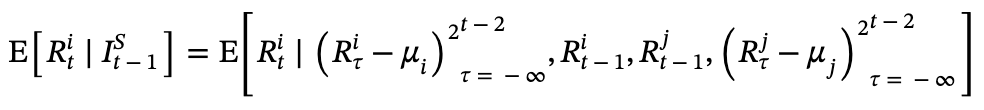
\includegraphics[scale=0.5]{granger_causality_1.png}
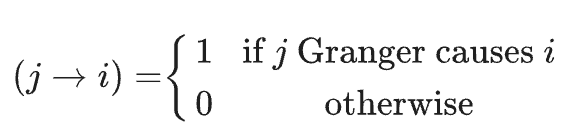
\includegraphics[scale=0.5]{granger_causality_2.png}

In general, if country \textit{j} causes volatility in country \textit{i}, then from \textit{j} to \textit{i} are connected in one direction. But, there is also a possibility in which country \textit{i} does not cause any volatility in country \textit{j}, indicating that the edge is only one direction. Lai \& Hu (2021) derived this formula to calculate the correlation of stock index volatility between two countries.

The Granger-causality approach to build networks was also used by Zhang et al. (2023) to analyze the systemic risk in global stock indexes during COVID-19 recession. This literature was taking Lai \& Hu (2021) as its foundation and trying to solve nonlinear relationships in systemic risk problems. As stated by Chen et al. (2013) and Etesami et al. (2017), econometric can be used as the groundwork of systemic risk analysis. However, one challenge in making it as close as possible to real-world scenarios is the non-linearity factor between metrics. Unfortunately, Lai \& Hu (2021) were not taking this factor into their consideration when making the network. Zhang et al. (2023) was introducing the non-linear Granger-causality to support such a scenario, making the network model more accurate. 

In another literature, Duan et al. (2020) were proposing to use volatility, leverage, and correlation factors to construct the network. Unlike Lai \& Hu (2021) and Zhang et al. (2023) that were using global stock indexes, the authors are using global bank data. To calculate the volatility and leverage for each bank in pre-covid and post-covid eras, they are using $\Delta$CoVaR that evaluates the growth rate of the market value of assets (Adrian \& Brunnermeier, 2016). As the market value of banks’ assets change over time, so does their leverage level in the interbank networks. Bigger leverage means new opportunities for banks to do more aggressive and riskier activities, exposing them to looming systemic risk (Adrian \& Brunnermeier, 2009). Furthermore, Duan et al. (2020) derived the $\Delta$CoVaR equation based on the situation during COVID outbreak and produce formula.

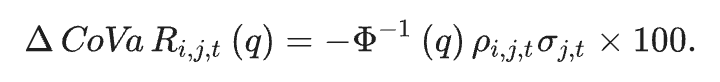
\includegraphics[scale=0.7]{covar.png}

This formula indicates that higher value of $\Delta$CoVaR means higher systemic value for bank \textit{q} as their assets’ growth is significant that the particular bank poses greater probability of collapsing under bad circumstances. During COVID, as financial activities halted across the globe, Duan et al. (2020) believed that assets’ lost their liquidity due to uncertainty in the market. The authors were using banks as the node and also using $\Delta$CoVaR value as the weight of the links between two banks.

As comparison of the usage of network science to analyze systemic risk of global recession, we also want to take a look into the 2007 great recession case. Markose et al. (2012) was using global banks data to construct their network using leverage and correlation. The authors were taking Credit Default Swap (CDS) count on residential mortgages as the representation of the leverage for each of the banks in both United States (US) and non-US intermediary financial institutions. The higher the count of CDS contracts that banks own, the higher the systemic risk that bank has. This comes to the fact that the buyer of a CDS does need to own any underlying security or have any credit exposure, thus making the bank to hedge the naked CDS buy position Markose et al. (2012). These were risky activities that banks were doing in hope for more profit.

On the other hand, Battiston et al. (2012) was proposing another approach to analyze the truth behind the aforementioned doctrine. They are using leverage and correlation factors as well to construct the network, but taking debt rank as the network metrics instead of CDS of residential mortgages. Although they are both referencing the risky position of the banks, debt rank is influenced by the sum amount of all activities that the bank does. So we can see debt rank as an overall overview of banks’ health while CDS is one of the factors that contribute to this health status. Both Markose et al. (2012) and Battiston et al. (2012) were using banks as the node and also using either CDS count and debt rank value as the weight of the links between two banks.

Unlike COVID recession, the 2007 great recession magnitude was tremendous because of the “too-big-to-fail” doctrine (Zhou, 2009). Banks were seen invulnerable to any risks due to the amount of assets that they had, thus giving them the “opportunity” to do risky businesses, something that exposed them to a far greater risk of collapsing. Both Markose et al. (2012) and Battiston et al. (2012) focused on unveiling the risk behind the “too-big-to-fail” doctrine from system topology and systemic risk point of view.

\subsection{Centrality}
As previously indicated, there are at least three centrality approaches that are available in network science to do systemic risk analysis; degree, closeness, and eigenvector. Each of these approaches has its own characteristics depending on the point of view that the network is representing.
For example, Lai \& Hu (2021) chose to use both degree and closeness centrality. As they build their network based on volatility correlation between countries, the higher the degree of a certain country means the higher the influence that particular country receives and emits. The authors also divided the degree into two categories that represent both the influence that countries take (in-degree) and also send out (out-degree), deepening the systemic risk analysis as it is not always reciprocal. What is interesting is that the authors’ reasoning on choosing the degree centrality as its first focus to do the analysis because it is the simplest centrality to be calculated yet brings sufficient preliminary information to the table. Due to the way authors constructed the network, the country with the highest in-degree held the most important information as they will be the country that is exposed the most by the systemic risk. On the other hand, the country with the highest out-degree can be seen as the largest domino piece that can potentially collapse the entire system if it falls. As further analysis, the authors also use closeness centrality to estimate the amount of time for systemic risk to propagate throughout the network. The country that has highest closeness centrality can reach out the furthest country in the network with only a few steps, meaning if this country collapses then the effect can be fast transmitted. Although closeness centrality is prone to bias on loosely connected networks and generally more computational expensive compared to degree centrality, the authors argued that the network that they built was fully connected and small in terms of size (number of nodes). 

In contrast to Lai \& Hu (2021), Zhang et al. (2023) were using eigenvector centrality instead of degree centrality, although they are also using closeness centrality. Unlike degree, closeness, and betweenness that focus on determining the centrality based on node’s attributes and locations, eigenvector centrality calculates the importance of the nodes based on the significance of all edges that connect to that particular node. Due to this particular reason, it is a good representation of measurement that the authors’ use to create the network, in this case Nonlinear Granger-causality. The higher the eigenvector centrality value means the stock index poses higher systemic risk in the system as they are seen as influential nodes in the network, which tiny disruption on these nodes can have ripple effects to the entire network (Zhang et al., 2023). 

Similar to Zhang et al. (2023), Duan et al. (2020) and Markose et al. (2012) were also using eigenvector centrality to analyze systemic risk in their bank network. However, unlike Zhang et al. (2023) and Lai \& Hu (2021), these authors were not using closeness centrality. Both Duan et al. (2020) and Markose et al. (2012) were using bank data and focus more on leverage and volatility of bank assets. Although the measurement taken by the authors differs, they want to highlight the measurement result in the centrality measurement. Therefore they were only using the eigenvector centrality to measure the systemic risk. Despite the same centrality measurement, the interpretation of the result is a little bit different. Duan et al. (2020) was using $\Delta$CoVaR to construct their network, which means high eigenvector value represented higher systemic value for that particular bank as their assets’ grew significantly and heavily influenced by other banks as they were deemed as big banks. Meanwhile in Markose et al. (2012) network, high eigenvector value represented higher systemic value for that particular bank as their bad debt in the form of CDS contracts was high. This means that particular bank was seen as a big bank and referenced by other banks for the number of CDS contracts they should own, increasing the systemic risk of the network even more.

Comparable to Markose et al. (2012), Battiston et al. (2012) was also using eigenvector centrality measurement for the same exact reason. However, they are also introducing a new approach on calculating centrality, called feedback centrality. Feedback centrality assesses the importance of nodes within a network by considering the feedback loops they participate in. It is particularly relevant in understanding how information or influence circulates within a network through iterative processes. Feedback centrality takes into account the potential for a node to receive feedback from its neighbors, contributing to its overall centrality. Since the author was using debt rank to construct their network, feedback centrality helps the author to measure the loop effect of borrow and lend activities of those banks. The higher the feedback centrality means the bank poses higher systemic risk in the system as they are in the loop of many debt cycles (Battiston et al., 2012).

\subsection{Clustering \& Modularity}
As previously stated, clustering approach is important to see the grouping pattern of the network and revealing the topology of the network itself. This is important for the systemic risk analysis as the grouping of nodes will increase the possibility of domino effect in case of crisis. As mentioned by Lai \& Hu (2021), clustering approach using clustering coefficient is critical to identify and quantify the possibility of crisis. The authors found a tendency for countries to group up together during COVID recession. They specified that there were at least three reasons behind such a phenomenon; close political contacts, frequent trade exchanges, and in-depth multi level cooperation mainly for COVID vaccine endeavor. The authors theorized that countries with high clustering coefficient were countries that had high overall systemic risk as they can easily trigger the ripple effect. One of the examples that authors gave was the US stock market crash was heavily influenced by South Korea stock market substantial decline. This further impacted European and other Asian stock indexes, thus triggering the global financial crisis.

Interestingly, Duan et al. (2020) was not using a clustering method to analyze systemic risk. The authors were heavily focussing on building the network using a complex finance model that can replicate real-world scenarios as closely as possible. Despite different approaches and dataset that the authors were using, they still managed to identify similar systemic fragility over the board due to across countries government policies and bank default risk channels. This is also the case in Zhang et al. (2023) in which they are not using any clustering methods to do systemic risk analysis. The authors were focussing more on introducing the nonlinearity segment to network creation, thus switching their focus more on the eigenvector centrality approach. The same as Duan et al. (2020), regardless of different methods and approaches, they still managed to acquire similar results. However, Duan et al. (2020) managed to conclude that the effect of covid recession had a more significant impact on macroeconomic variables, with more severe shocks to economic activity than the 2007 great recession. This statement was also found in other sectors including supply chain disruptions (Li et al., 2022, Golan et al., 2020).

The same as Lai \& Hu (2021), Markose et al. (2012) was also taking the clustering coefficient as one of the factors to analyze the systemic risk. The authors found out the high clustering phenomena of small world networks along with a sparse adjacency matrix in the banks’ CDS activity. They also revealed the CDS network in 2007 was clustered and concentrated, thus exposing the entire network to a great risk of collapsing. Due to the shape of the topology, the authors deduced that the structure has some capacity for containment of contagion and can have some stabilizing effects compared to the unstructured random graphs. Yet, the authors expressed that the magnitude of potential losses stemming from the failure of highly interconnected financial intermediaries surpassed their ability to fully internalize.

On the other hand, Battiston et al. (2012) was not using any clustering methods to do their systemic risk analysis. The reasoning behind it is the same as Duan et al. (2020) and Zhang et al. (2023), as all of them were focussing more on the financial model that they use to base the network on rather than in-depth analysis of the aforementioned networks. In Battiston et al. (2012) literature, they are building a financial model called debt rank and using both eigenvector and feedback centrality to reveal hidden information in the network. In spite of the difference, both Markose et al. (2012) and Battiston et al. (2012) still managed to debunk the “too-big-to-fail” doctrine (Zhou, 2009).

The evolution of clustering coefficient over time is also important to see the dynamic of the real-world and predict the fast coming recession, giving early warning so all parties can adapt to the situation and danger. As also shown by Lai \& Hu (2021), there was a pattern change before and after March 2020. Before COVID hits, the network was built with the USA, Japan, UK, Germany, and Russia as its core and the rest of the world surrounding them. However, this pattern shifted after March 2020, in which clustering coefficients for all stock indexes were raised and made the network more connected slowly over time. This phenomenon was due to the vaccine endeavor that was going on at that moment of time. According to Lai \& Hu (2021), analyzing nodes that have high clustering coefficients is critical to forecast the possibility of a crisis, and we can always start from the powerhouse of the global economy such as G20 countries. The evolution of clustering coefficient can also be observed in Markose et al. (2012) literature. The authors found that the clustering coefficient is at its lowest point after the great recession struck, but then slowly getting up to the point it was even higher in 2008. The authors stated that further experiment and analysis was needed to answer the type of countermeasures and adaptation moves that banks, governments, and financial institutions need to take.

\section{Summary \& Conclusion}
This section will contain the summary from multiple approaches for systemic risk analysis in stock market

\section{Future Work}
This section will contain the potential future work for systemic risk analysis in stock market

%                Now build the reference list
\bibliographystyle{unsrt}   % The reference style
%                This is plain and unsorted, so in the order
%                they appear in the document.


\small
\bibliography{main}       % bib file(s).

\end{document}

